%!TeX encoding = UTF-8
%!TeX program = xelatex
\documentclass[notheorems, aspectratio=54]{beamer}
% aspectratio: 1610, 149, 54, 43(default), 32

\usepackage{latexsym}
\usepackage{amsmath,amssymb}
\usepackage{mathtools}
\usepackage{color,xcolor}
\usepackage{graphicx}
\usepackage{algorithm}
\usepackage{amsthm}
\usepackage{lmodern} % 解决 font warning
% \usepackage[UTF8]{ctex}
\usepackage{animate} % insert gif
\usepackage{lipsum} % To generate test text 
\usepackage{ulem} % 下划线,波浪线
\usepackage{autobreak}
\usepackage{multirow}
\usepackage{enumerate}
\usepackage{textcomp}
\usepackage{subfigure}




\usepackage{listings} % display code on slides; don't forget [fragile] option after \begin{frame}

% --------------- function-------------------------------
% tikx
\usepackage{framed}
\usepackage{tikz}
\usepackage{pgf}
\usetikzlibrary{calc,trees,positioning,arrows,chains,shapes.geometric,%
	decorations.pathreplacing,decorations.pathmorphing,shapes,%
	matrix,shapes.symbols}
\pgfmathsetseed{1} % To have predictable results
% Define a background layer, in which the parchment shape is drawn
\pgfdeclarelayer{background}
\pgfsetlayers{background,main}

% define styles for the normal border and the torn border
\tikzset{
	normal border/.style={orange!30!black!10, decorate, 
		decoration={random steps, segment length=2.5cm, amplitude=.7mm}},
	torn border/.style={orange!30!black!5, decorate, 
		decoration={random steps, segment length=.5cm, amplitude=1.7mm}}}

% Macro to draw the shape behind the text, when it fits completly in the
% page
\def\parchmentframe#1{
	\tikz{
		\node[inner sep=2em] (A) {#1};  % Draw the text of the node
		\begin{pgfonlayer}{background}  % Draw the shape behind
			\fill[normal border] 
			(A.south east) -- (A.south west) -- 
			(A.north west) -- (A.north east) -- cycle;
\end{pgfonlayer}}}

% Macro to draw the shape, when the text will continue in next page
\def\parchmentframetop#1{
	\tikz{
		\node[inner sep=2em] (A) {#1};    % Draw the text of the node
		\begin{pgfonlayer}{background}    
			\fill[normal border]              % Draw the ``complete shape'' behind
			(A.south east) -- (A.south west) -- 
			(A.north west) -- (A.north east) -- cycle;
			\fill[torn border]                % Add the torn lower border
			($(A.south east)-(0,.2)$) -- ($(A.south west)-(0,.2)$) -- 
			($(A.south west)+(0,.2)$) -- ($(A.south east)+(0,.2)$) -- cycle;
\end{pgfonlayer}}}

% Macro to draw the shape, when the text continues from previous page
\def\parchmentframebottom#1{
	\tikz{
		\node[inner sep=2em] (A) {#1};   % Draw the text of the node
		\begin{pgfonlayer}{background}   
			\fill[normal border]             % Draw the ``complete shape'' behind
			(A.south east) -- (A.south west) -- 
			(A.north west) -- (A.north east) -- cycle;
			\fill[torn border]               % Add the torn upper border
			($(A.north east)-(0,.2)$) -- ($(A.north west)-(0,.2)$) -- 
			($(A.north west)+(0,.2)$) -- ($(A.north east)+(0,.2)$) -- cycle;
\end{pgfonlayer}}}

% Macro to draw the shape, when both the text continues from previous page
% and it will continue in next page
\def\parchmentframemiddle#1{
	\tikz{
		\node[inner sep=2em] (A) {#1};   % Draw the text of the node
		\begin{pgfonlayer}{background}   
			\fill[normal border]             % Draw the ``complete shape'' behind
			(A.south east) -- (A.south west) -- 
			(A.north west) -- (A.north east) -- cycle;
			\fill[torn border]               % Add the torn lower border
			($(A.south east)-(0,.2)$) -- ($(A.south west)-(0,.2)$) -- 
			($(A.south west)+(0,.2)$) -- ($(A.south east)+(0,.2)$) -- cycle;
			\fill[torn border]               % Add the torn upper border
			($(A.north east)-(0,.2)$) -- ($(A.north west)-(0,.2)$) -- 
			($(A.north west)+(0,.2)$) -- ($(A.north east)+(0,.2)$) -- cycle;
\end{pgfonlayer}}}

% Define the environment which puts the frame
% In this case, the environment also accepts an argument with an optional
% title (which defaults to ``Example'', which is typeset in a box overlaid
% on the top border
\newenvironment{parchment}[1][Example]{%
	\def\FrameCommand{\parchmentframe}%
	\def\FirstFrameCommand{\parchmentframetop}%
	\def\LastFrameCommand{\parchmentframebottom}%
	\def\MidFrameCommand{\parchmentframemiddle}%
	\vskip\baselineskip
	\MakeFramed {\FrameRestore}
	\noindent\tikz\node[inner sep=1ex, draw=black!20,fill=white, 
	anchor=west, overlay] at (0em, 2em) {\sffamily#1};\par}%
{\endMakeFramed}

% ----------------------------------------------

\mode<presentation>{
	\usetheme{CambridgeUS}
	% Boadilla CambridgeUS
	% default Antibes Berlin Copenhagen
	% Madrid Montpelier Ilmenau Malmoe
	% Berkeley Singapore Warsaw
	\usecolortheme{beaver}
	% beetle, beaver, orchid, whale, dolphin
	\useoutertheme{infolines}
	% infolines miniframes shadow sidebar smoothbars smoothtree split tree
	\useinnertheme{circles}
	% circles, rectanges, rounded, inmargin
}
% 设置 block 颜色
\setbeamercolor{block title}{bg=red!30,fg=white}

\newcommand{\reditem}[1]{\setbeamercolor{item}{fg=red}\item #1}

% 缩放公式大小
\newcommand*{\Scale}[2][4]{\scalebox{#1}{\ensuremath{#2}}}

% 解决 font warning
\renewcommand\textbullet{\ensuremath{\bullet}}

% ---------------------------------------------------------------------
% flow chart
\tikzset{
	>=stealth',
	punktchain/.style={
		rectangle, 
		rounded corners, 
		% fill=black!10,
		draw=white, very thick,
		text width=6em,
		minimum height=2em, 
		text centered, 
		on chain
	},
	largepunktchain/.style={
		rectangle,
		rounded corners,
		draw=white, very thick,
		text width=10em,
		minimum height=2em,
		on chain
	},
	line/.style={draw, thick, <-},
	element/.style={
		tape,
		top color=white,
		bottom color=blue!50!black!60!,
		minimum width=6em,
		draw=blue!40!black!90, very thick,
		text width=6em, 
		minimum height=2em, 
		text centered, 
		on chain
	},
	every join/.style={->, thick,shorten >=1pt},
	decoration={brace},
	tuborg/.style={decorate},
	tubnode/.style={midway, right=2pt},
	font={\fontsize{10pt}{12}\selectfont},
}
% ---------------------------------------------------------------------

% code setting
\lstset{
	language=C++,
	basicstyle=\ttfamily\footnotesize,
	keywordstyle=\color{red},
	breaklines=true,
	xleftmargin=2em,
	numbers=left,
	numberstyle=\color[RGB]{222,155,81},
	frame=leftline,
	tabsize=4,
	breakatwhitespace=false,
	showspaces=false,               
	showstringspaces=false,
	showtabs=false,
	morekeywords={Str, Num, List},
}

% ---------------------------------------------------------------------

%% preamble
\title[Suggestions for Retaurants]{\LARGE\textbf{{How to Improve Your Restaurant?}}}
% \subtitle{The subtitle}
\author[L.Du, L.Ma, W.Xie]{Lize Du, Linquan Ma, Wenjia Xie}
\institute{STAT 628}

% -------------------------------------------------------------

\begin{document}
	
	%% title frame
	\begin{frame}
	\titlepage
\end{frame}

%% normal frame
\begin{frame}
\frametitle{Outline}
\begin{itemize}
	\item[\textcolor{darkred}{\textbullet}] Star Prediction
	\vspace{2ex}
	
	\item[\textcolor{darkred}{\textbullet}] Analyze Methods
	\begin{itemize}
		\item[\textcolor{darkred}{1}] Nouns in Reviews
		\item[\textcolor{darkred}{2}] Attributes
	\end{itemize}
	\vspace{2ex}
	
	\item[\textcolor{darkred}{\textbullet}] Suggestions for Traditional American Restaurants
	\begin{itemize}
		\item[\textcolor{darkred}{1}] Food
		\item[\textcolor{darkred}{2}] Environment
		\item[\textcolor{darkred}{3}] Service
		\item[\textcolor{darkred}{4}] Facility
	\end{itemize}
\end{itemize}

\end{frame}

\begin{frame}
\frametitle{Star Prediction}
\ \ \ \ \ \ Data: \ \ Over 5 million reviews
\vspace{3ex}

\ \ \ \ \ \ Method: \ \  Logistic regression
\vspace{3ex}

\ \ \ \ \ \ RMSE: \ \ 91.986\%
\vspace{3ex}

\end{frame}

\begin{frame}
\frametitle{Nouns in Reviews}
\ \ \ \ 1. Remain the words whose \textcolor{darkred}{frequency} larger than 4000, after this process, we have 1767 words left.
\vspace{1.5ex}

\ \ \ \ 2. Use \textcolor{darkred}{information gain} to rank the words, choose top 1000 words.
\vspace{1.5ex}

\ \ \ \ 3. Choose nouns using \textcolor{darkred}{$nltk.pos\_tag$ method} and in the end we have 603 nouns left.
\vspace{1.5ex}

\ \ \ \ 4. Use all the review data of Traditional American Restaurants and the 603 nouns to build a \textcolor{darkred}{linear model}.
\vspace{1.5ex}

\ \ \ \ 5. Use \textcolor{darkred}{bootstrap} to calculate the standard deviation of each word's coefficient in our model by rebuilding the model using random sample (size = 10000 observations) 1000 times.
\vspace{1.5ex}

\ \ \ \ 6. Rank the word by \textcolor{darkred}{coefficient/sd}, focus on the top 100 positive and negative words and choose some informative words manually.

\end{frame}

\begin{frame}
\frametitle{Attributes}

\ \ \ \ Attributes are from the "business" dataset that reflect various characteristics of the restaurants.
\vspace{2ex}

\ \ \ \ There are \textcolor{darkred}{39} attributes in the dataset recording different aspects, such as "garage", "street", "validated", "lot" and "valet" in the "Business parking" attribute. We changed all the sub-attributes into independent columns and get \textcolor{darkred}{66} different attributes in total. 
\vspace{2ex}

\ \ \ \ However, "accept insurance", "byob" and "restaurants counter service" only has one level. Hence we drop them from our analysis. A list of most important attributes for improving the stars are selected based on \textcolor{darkred}{CART} and \textcolor{darkred}{ANOVA}.

\end{frame}

\begin{frame}
\frametitle{Classification and Regression Trees (CART)}
\begin{itemize}
	\item[\textcolor{darkred}{\textbullet}] Missing data
	
	\vspace{2ex}
	
	\ \ \ \ The overall missing rate is around 0.5, first drop the attributes whose missing rate is greater than 0.5. Then we have 36 attributes left with overall missing rate 16.5\%. 
\vspace{2ex}

	\ \ \ \ The R package $rpart$ applies surrogate splits to deal with missing data comfortably. With $rpart$, we can directly applies the dataset with missing values to the rpart function.
\end{itemize}


\end{frame}

\begin{frame}
\frametitle{Classification and Regression Trees (CART)}

\begin{figure}
    \centering
    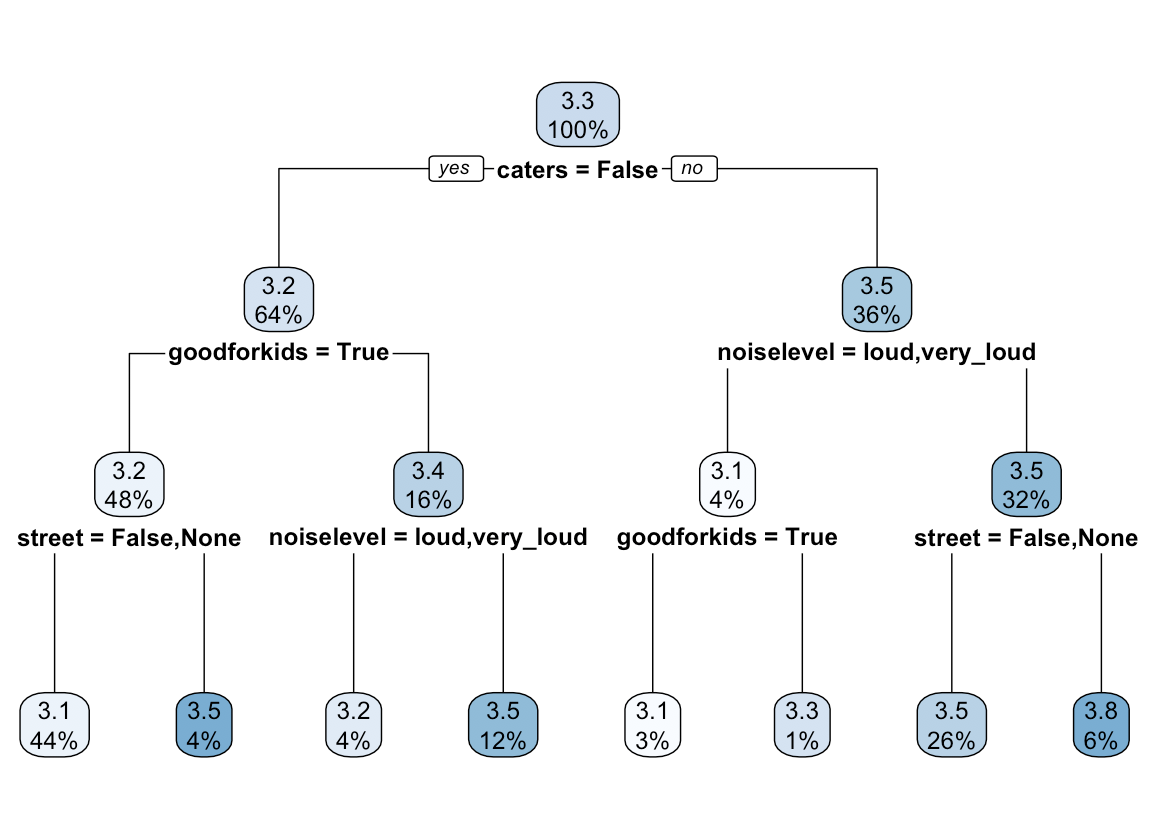
\includegraphics[width=4.5in]{rpart_tree.png}
\end{figure}
\end{frame}

\begin{frame}
\frametitle{ANOVA test}
 \ \ \ \ 1. Performed one-way ANOVA marginally for each attribute to see if an attribute is significant. 
 \vspace{2ex}
 
 \ \ \ \ 2. Ranked the p-values of each attribute from lowest to the highest, to discover that the previously top 5 attributes selected using rpart have the top 10 smallest p-values. 
 \vspace{2ex} 
 
 \ \ \ \ 3. Confirms that the top 5 attributes are important indicators for review stars.
\end{frame}


\begin{frame}
\frametitle{Food}

\begin{figure}
	\begin{minipage}[t]{0.5\linewidth}
		\centering
		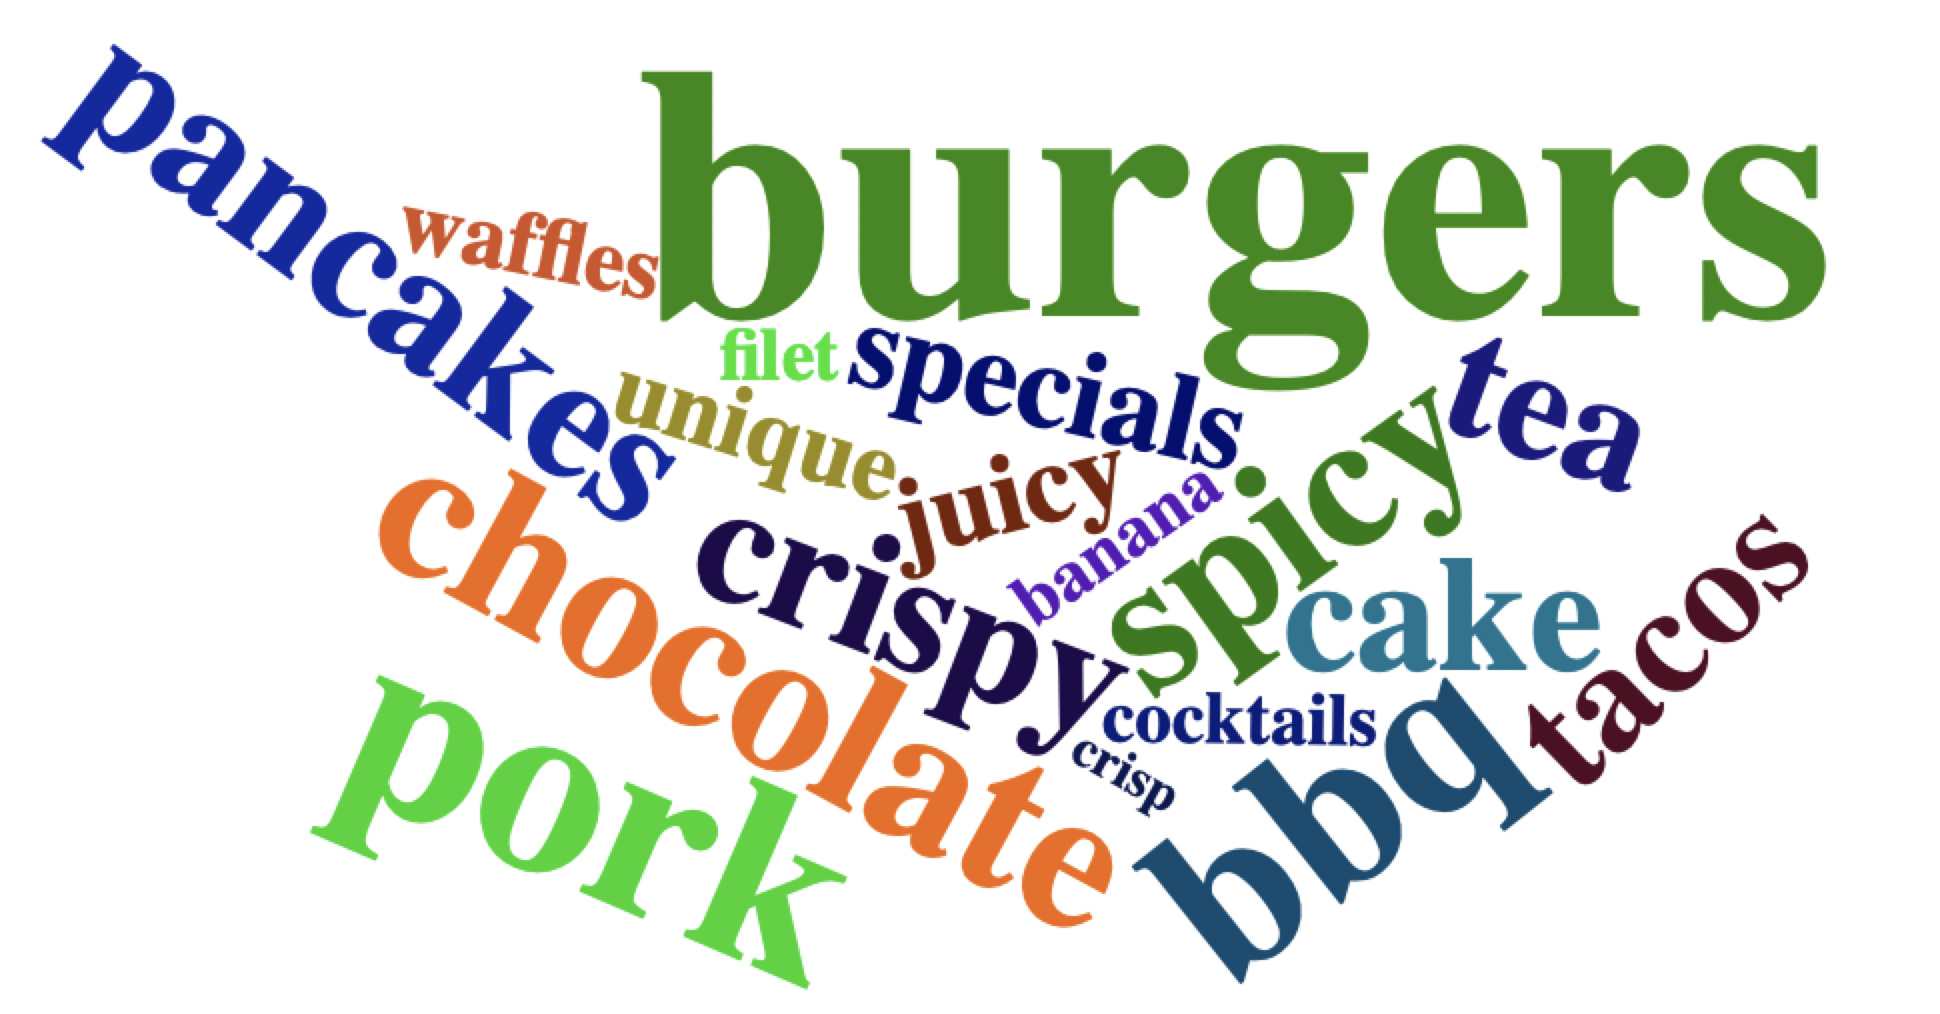
\includegraphics[width=2.2in]{food_good.png}
		\caption{Positive Foods}
		\label{fig:side:a}
	\end{minipage}%
	\begin{minipage}[t]{0.5\linewidth}
		\centering
		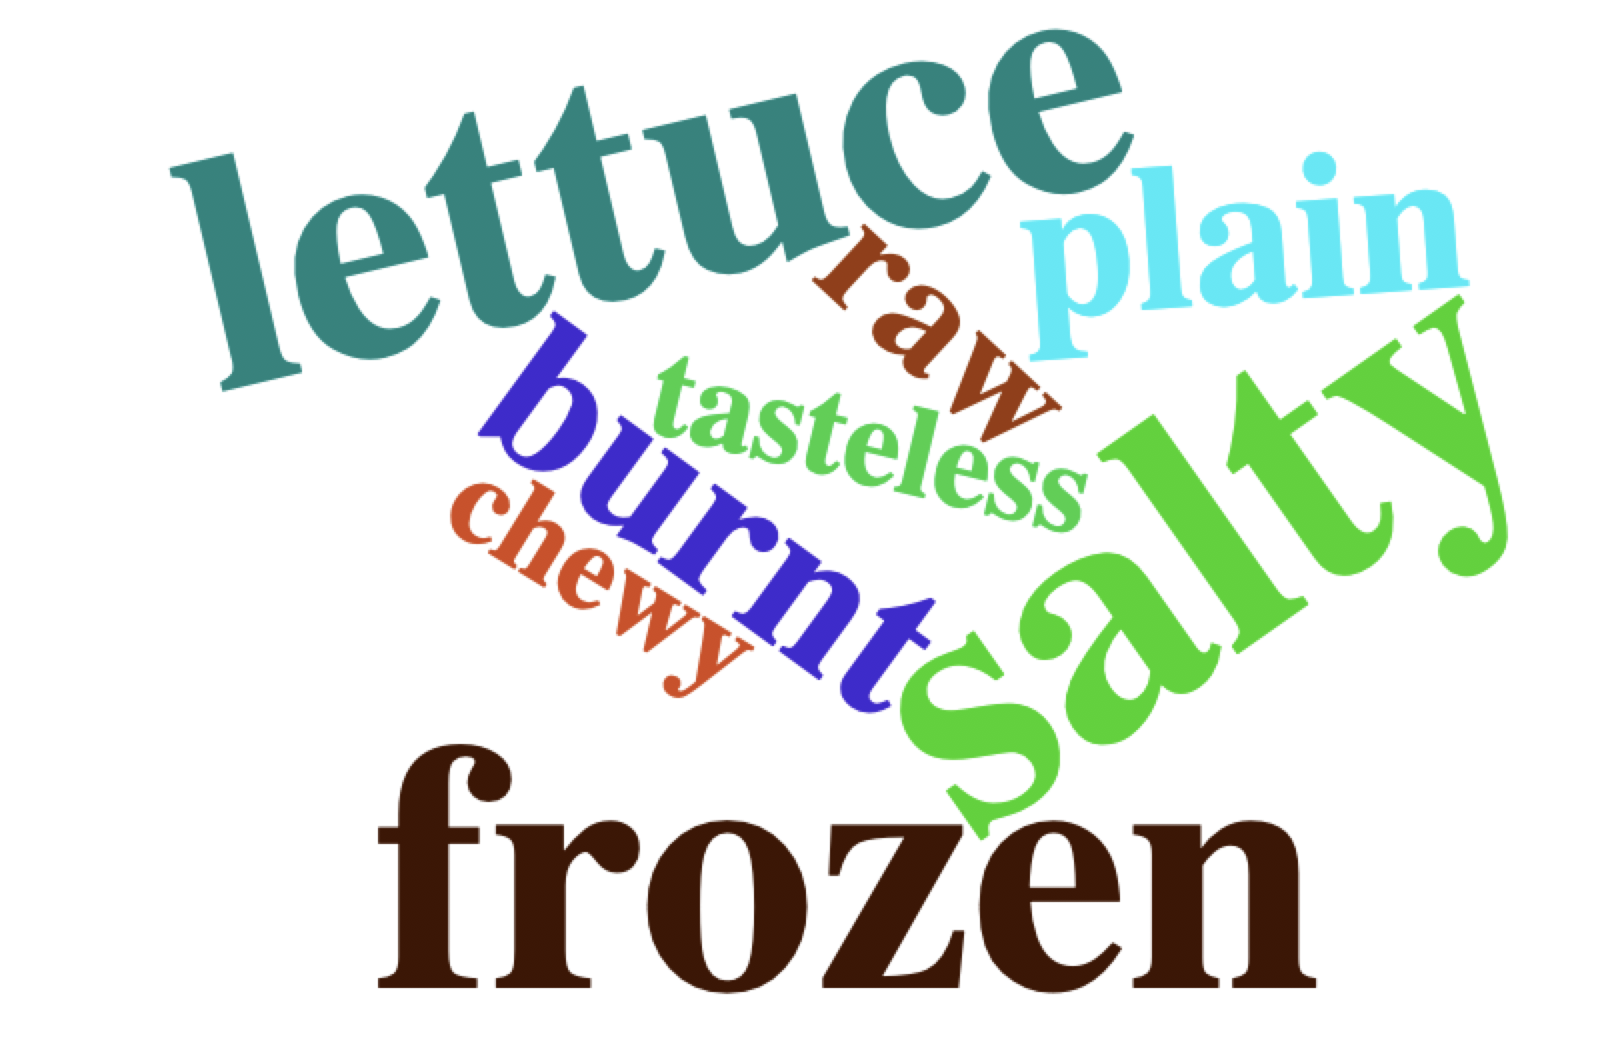
\includegraphics[width=2.2in]{food_bad.png}
		\caption{Negative Foods}
		\label{fig:side:b}
	\end{minipage}
\end{figure}
\end{frame}

\begin{frame}
\frametitle{Food}
\ \ \ \ You'd better have
\begin{itemize}
	\item[\textcolor{darkred}{\textbullet}] Menu: Include burgers, pancakes, pork, tacos, filet and bbqs;
	\item[\textcolor{darkred}{\textbullet}] Meat: Juicy and crispy;
	\item[\textcolor{darkred}{\textbullet}] Dessert: Cakes, waffles or chocolates;
	\item[\textcolor{darkred}{\textbullet}] Drinks: Tea and cocktails;
	\item[\textcolor{darkred}{\textbullet}] Specials on your menu every few days.
\end{itemize}
\vspace{2ex}

\ \ \ \ What you should take care of is you shouldn't make the food too salty, too chewy or even burnt, raw, frozen or tasteless food. 

\ \ \ \ Another tip is you should know if the customer wants lettuce in their sandwisches and burgers and they want what knid of lettuce in it.

\end{frame}

\begin{frame}
\frametitle{Environment}
\begin{figure}
	\begin{minipage}[t]{0.5\linewidth}
		\centering
		
\includegraphics[width=2.2in]{environment_good.png}
		\caption{Positive Environment}
		\label{fig:side:a}
	\end{minipage}%
	\begin{minipage}[t]{0.5\linewidth}
		\centering
		
\includegraphics[width=2.2in]{environment_bad.png}
		\caption{Negative Environment}
		\label{fig:side:b}
	\end{minipage}
\end{figure}
\end{frame}

\begin{frame}
\frametitle{Environment}
\ \ \ \ You'd better
\begin{itemize}
	\item[\textcolor{darkred}{\textbullet}] Keep everything in their places all the time;
	\item[\textcolor{darkred}{\textbullet}] Come up with some ideas to make people eating here happily;
	\item[\textcolor{darkred}{\textbullet}] Prepare some big tables because some people may come with their family;
	\item[\textcolor{darkred}{\textbullet}] Keep the restroom clean all the time;
	\item[\textcolor{darkred}{\textbullet}] Make the air in your restaurant fresh;
	\item[\textcolor{darkred}{\textbullet}] Keep the noise level low.
\end{itemize}

\end{frame}

\begin{frame}
\frametitle{Service}
\begin{figure}
	\begin{minipage}[t]{0.5\linewidth}
		\centering
		
\includegraphics[width=2.2in]{staff_good.png}
		\caption{Positive Service}
		\label{fig:side:a}
	\end{minipage}%
	\begin{minipage}[t]{0.5\linewidth}
		\centering
		
\includegraphics[width=2.2in]{staff_bad.png}
		\caption{Negative Service}
		\label{fig:side:b}
	\end{minipage}
\end{figure}
\end{frame}

\begin{frame}
\frametitle{Service}
\ \ \ \ You'd better
\begin{itemize}
	\item[\textcolor{darkred}{\textbullet}] Train your employees well so that they can properly answer customers' questions and satisfy their requests, such as give the customers right recommendations.
	\item[\textcolor{darkred}{\textbullet}] Prepare food quickly;
	\item[\textcolor{darkred}{\textbullet}] Smile to customers;
	\item[\textcolor{darkred}{\textbullet}] Make your team professional to serve with loves.
\end{itemize}

\end{frame}

\begin{frame}
\frametitle{Facility}
\ \ \ \ You'd better prepare
\begin{itemize}
	\item[\textcolor{darkred}{\textbullet}] Caters;
	\item[\textcolor{darkred}{\textbullet}] Parking lots, especially street parking;
	\item[\textcolor{darkred}{\textbullet}] Facilities that are good for kids, such as children seats;
	\item[\textcolor{darkred}{\textbullet}] Restaurants delivery.
\end{itemize}
\end{frame}

\begin{frame}
\frametitle{Advantages and Disadvantages}
\begin{itemize}
	\item[\textcolor{darkred}{\textbullet}] Advantages
	\begin{itemize}
		\item[\textcolor{darkred}{1}] For reviews, we focus on nouns and the result seems reasonable.
		\item[\textcolor{darkred}{2}] For business, we use both ANOVA and Cart tree method to calculate the importance of features, which is reliable.
	\end{itemize}
\vspace{2ex}

	\item[\textcolor{darkred}{\textbullet}] Disadvantages
	\begin{itemize}
		\item[\textcolor{darkred}{1}] For the prediction model, we only use logistic regression with 2000 covariates which can not predict too well.
		\item[\textcolor{darkred}{2}] We are not able to quantify the effect of wach word or feature to the rate of review.
	\end{itemize}
\end{itemize}

\end{frame}

\begin{frame}
\begin{figure}[H]
	\centering
	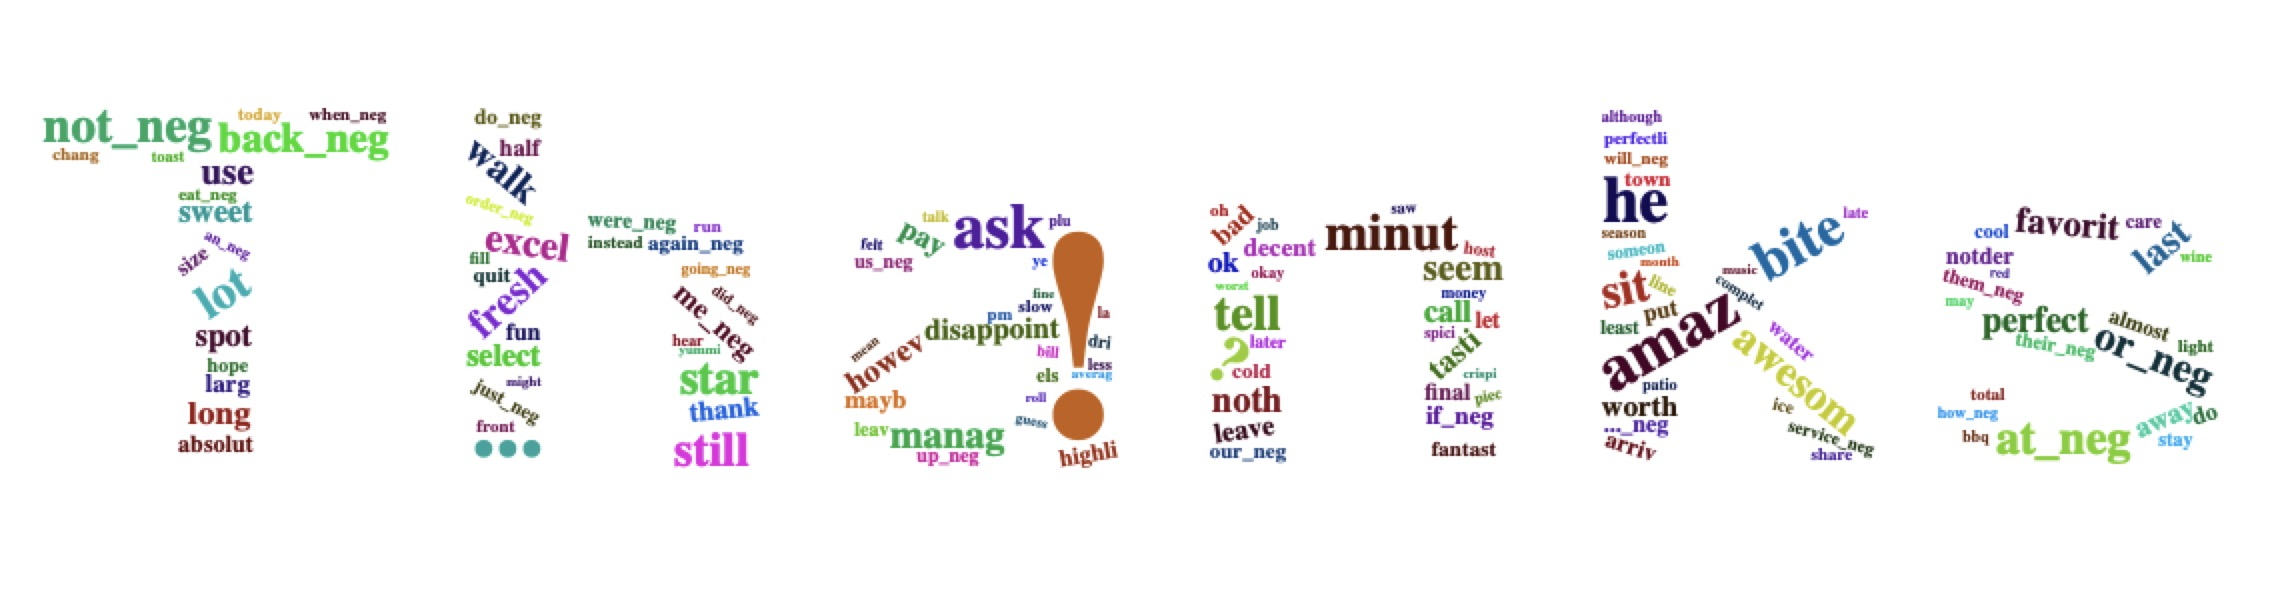
\includegraphics[width=4.6in]{thanks.jpg}
\end{figure}
\end{frame}
\end{document}